\documentclass[12pt, a4paper, oneside]{ctexart}
\usepackage{amsmath, amsthm, amssymb, bm, color, graphicx, geometry, mathrsfs,extarrows, braket, booktabs, array}
\usepackage[colorlinks,linkcolor=red,anchorcolor=blue,citecolor=blue,urlcolor=blue,menucolor=black]{hyperref}
\setmainfont{Times New Roman}  % 设置英文字体
\setsansfont{Calibri}
\setmonofont{Consolas}

\linespread{1.4}
%\geometry{left=2.54cm,right=2.54cm,top=3.18cm,bottom=3.18cm}
\geometry{left=1.84cm,right=1.84cm,top=2.18cm,bottom=2.18cm}
\newenvironment{problem}{\par\noindent\textbf{题目. }}{\bigskip\par}
\newenvironment{solution}{\par\noindent\textbf{解答. }}{\bigskip\par}
\newenvironment{note}{\par\noindent\textbf{注记. }}{\bigskip\par}

%%%% 图片相对路径 %%%%
\graphicspath{{figure/}} % 当前目录下的figure文件夹, {../figure/}则是父目录的figure文件夹

\everymath{\displaystyle} % 默认全部行间公式
\DeclareMathOperator*\uplim{\overline{lim}} % 定义上极限 \uplim_{}
\DeclareMathOperator*\lowlim{\underline{lim}} % 定义下极限 \lowlim_{}
\let\leq=\leqslant % 将全部leq变为leqslant
\let\geq=\geqslant % geq同理

% 一些宏定义
\def\arg{\text{Arg}}
\def\bd{\boldsymbol}    % 加粗(向量) boldsymbol
\def\disp{\displaystyle}% 使用行间公式 displaystyle(默认)
\def\tsty{\textstyle}   % 使用行内公式 textstyle
\def\sign{\text{sign}}  % sign function
\def\wtd{\widetilde}    % 宽波浪线 widetilde
\def\res{\text{Res}}
\def\R{\mathbb{R}}      % Real number
\def\C{\mathbb{C}}      % Complex number
\def\N{\mathbb{N}}      % Complex number
\def\d{\mathrm{d}}      % differential operator
\def\e{\mathrm{e}}      % Euler's number
\def\i{\mathrm{i}}      % imaginary number
\def\re{\mathrm{Re\,}}    % Real part
\def\im{\mathrm{Im\,}}    % Imaginary part
\def\L{\mathcal{L}}     % Loss function
\def\wdh{\widehat}      % 宽帽子 widehat
\def\ol{\overline}      % 上横线 overline
\def\ul{\underline}     % 下横线 underline
\def\add{\vspace{1ex}}  % 增加行间距
\def\del{\vspace{-3.5ex}}  % 减少行间距

% 基本信息
\newcommand{\RQ}{\today} % 日期
\newcommand{\km}{复变函数} % 科目
\newcommand{\bj}{强基数学002} % 班级
\newcommand{\xm}{吴天阳} % 姓名
\newcommand{\xh}{2204210460} % 学号

\begin{document}

%\pagestyle{empty}
\pagestyle{plain}
\vspace*{-15ex}
\centerline{\begin{tabular}{*5{c}}
    \parbox[t]{0.25\linewidth}{\begin{center}\textbf{日期}\\ \large \textcolor{blue}{\RQ}\end{center}} 
    & \parbox[t]{0.2\linewidth}{\begin{center}\textbf{科目}\\ \large \textcolor{blue}{\km}\end{center}}
    & \parbox[t]{0.2\linewidth}{\begin{center}\textbf{班级}\\ \large \textcolor{blue}{\bj}\end{center}}
    & \parbox[t]{0.1\linewidth}{\begin{center}\textbf{姓名}\\ \large \textcolor{blue}{\xm}\end{center}}
    & \parbox[t]{0.15\linewidth}{\begin{center}\textbf{学号}\\ \large \textcolor{blue}{\xh}\end{center}} \\ \hline
\end{tabular}}
\vspace*{4ex}

% 正文部分
\paragraph{第六章\ 2.}求下列积分: (1)$\int_{|z| = 1}\frac{\,\d z}{z^3(z^2-2)};$

(2)$\int_{|z| = R}\sqrt{(z-a)(z-b)}\,\d z\quad(a\neq b,\ R > \max(|a|, |b|).$
\begin{solution}
    (1) $\int_{|z| = 1}\frac{\d z}{z^3(z^2-2)} = 2\pi \i\res(f, 0) = \left(\frac{1}{z^2-2}\right)^{(2)}\biggl|_{z=0} = -\frac{\pi\i}{2}.$
\end{solution}
\paragraph{5.}设$\varphi(z)$在$z=a$点解析, $\varphi'(a)\neq 0$, 证明:
\begin{equation*}
    \frac{A}{\varphi'(a)}=\frac{1}{2\pi\i}\int_{|z-a|=\rho}\frac{A}{\varphi(z)-\varphi(a)}\,\d z\quad (\rho\text{充分小,}A\text{为常数}).
\end{equation*}
\begin{proof}
    \begin{equation*}
        \frac{1}{2\pi\i}\int_{|z-a|=\rho}\frac{A}{\varphi(z)-\varphi(a)}\,\d z = \frac{1}{2\pi\i}\int_{|z-a|=\rho}\frac{A}{\frac{\varphi(z)-\varphi(a)}{z-a}(z-a)}\,\d z = \frac{1}{2\pi\i}\int_{|z-a|=\rho}\frac{A}{\varphi'(a)(z-a)}\,\d z = \frac{A}{\varphi'(a)}t
    \end{equation*}
\end{proof}
\paragraph{6.}设$\varphi(z)$在$z=a$点解析, 且$\varphi'(a) \neq 0$, $\zeta_0=\varphi(a)$是函数$f(\zeta)$的简单极点, 其留数为$A$, 求$\res(f\circ \varphi;a)$.
\begin{solution}由$\varphi$在$z=a$的邻域内连续, 由反函数求导公式$\d(\zeta^{-1})(z) = \frac{\d \zeta}{\varphi'(\zeta)}$可知
    \begin{equation*}
        \frac{1}{2\pi\i}\int_{|z-a|=\rho}f(\varphi(z))\,\d z\xlongequal{\varphi^{-1}}\frac{1}{2\pi\i}\int_{|z-\zeta_0|=\rho_1}\frac{f(\zeta)}{\varphi'(\zeta)}\,\d \zeta = \frac{A}{\varphi'(\zeta_0)}.
    \end{equation*}
\end{solution}\del\del
\paragraph{7.}若$f(z)$是偶函数, 且是$\C$上亚纯函数, 证明:

(1) $\res(f;a) = -\res(f;-a)$;\add

(2) $\int_{|z|=R}f(z)\,\d z=0,\ f(z)$在$|z|=R$上无极点.

\begin{proof}
    (1)\del
    \begin{align*}
        \res(f;a)=&\ \frac{1}{2\pi\i}\int_{|z-a|=\rho}f(z)\,\d z\xlongequal{z=-\zeta}-\frac{1}{2\pi\i}\int_{|z+a|=\rho}f(-z)\,\d z\\
        \xlongequal{f\text{为偶函数}}&\ -\frac{1}{2\pi\i}\int_{|z+a|=\rho}f(z)\,\d z=-\res(f;-a).
    \end{align*}

    (2) 由于$f(z)$为$\C$上的亚纯函数, 则$f$在$|z|=R$所围成的区域$D$中的极点个数是有限的, 又由于$f$是偶函数, 所以极点也是对称的, 设极点为$z_1,z_2,\cdots, z_n, -z_1, -z_2, \cdots, -z_n$, 由留数定理和第一问结论得
    \begin{equation*}
        \int_{|z| = R}f(z)\,\d z=\sum_{k=1}^n\res(f; z_i)+\sum_{k=1}^n\res(f;-z_i) \xlongequal{(1)} 0
    \end{equation*}
\end{proof}
\paragraph{9.}求方程$x^5+11z+9=0$在下列区域内根的个数:

(1) $3/4<|z|<1;$\quad(2) $1<|z|<2$;\quad(3) $x>0, y>0$;\quad(4) $x<0, y>0$.

\begin{solution}
    (1) (2) 当$|z| = 3/4$时, $|z^5+11z|\leq 9$, 于是$z^5+11z+9$与$9$在$|z| \leq 3/4$上的根数相同;
    
    当$|z| = 1$时, $|z^5+9|= 10 < 11 = |11z|$,  于是$z^5+11z+9$与$11z$在$|z| < 1$上的根数相同, 均为$1$个根;
    
    当$|z| = 2$时, $|11z+9|=31 < 32 = |z^5|$, 于是$z^5+11z+9$与$z^5$在$|z|<2$上根数相同均为$5$个根.

    综上, $z^5+11z+9$在$3/4<|z|<1$上有$1$个根, 在$1<|z|<2$上有$4$个根.

    (3) 下面讨论第一象限上的根的个数, 做图6-2的曲线$\gamma = \gamma_1+\gamma_2+\gamma_3$, 设$P(z) = z^5+11z+9$, 则$P(x)\neq 0,\ (x > 0, x\in\R)$, 且$P(iy) = iy^5+11iy+9\neq 0$, 所以当$R\to\infty$时, $P(z)$在$\gamma$上无零点. 于是当$R\to\infty$时, 有
    \begin{align*}
        &\ \Delta_{\gamma_1}\arg(P(z)) = \arg(P(R) - P(0)) = \arg(R^5+11R+9)= 0\\
        &\ \Delta_{\gamma_2}\arg(P(z)) = \Delta_{\gamma_2}\arg(z^5(1+\frac{11z+9}{z^5})) = 2\pi +\frac{\pi}{2}+o(1)\\
        &\ \Delta_{\gamma_3}\arg(P(z)) = \arg(P(0) - P(iR)) = -\arg(9+iR(R^4+11)) = -\frac{\pi}{2}+o(1)
    \end{align*}
    所以 $\Delta_{\gamma} = \sum_{k=1}^3\Delta_{\gamma_k}\arg(P(z)) = 2\pi+o(1)\quad(R\to\infty)$. 由辐角原理知, $P(z)$在第一象限上只有一个根.

    (4) 由于$P(z)$在第一象限上有一个根, 有共轭性质, 在第四象限上也有一个根, 由(1)问可知, $P(z)$在$(-1,-3/4)$上有一个根, 且在$(\infty, -1]$上无根(根据导数恒正易得), 所以$P(z)$在第二和第三象限上各有一个根.
\end{solution}
\paragraph{11.}证明方程$z^8+3z^3+7z+5=0$在第一象限恰有两个根.
\begin{proof}
    做图6-2的曲线$\gamma = \gamma_1+\gamma_2+\gamma_3$, 设$P(z) = z^8+3z^3+7z+5=0$, 则$P(z)$在$\R_{\geq 0}$上无根, $P(iy) = y^8+5+i(7y-3y^3)\neq 0$, 所以当$R\to\infty$时, $P(z)$在$\gamma$上无根. 于是当$R\to\infty$时
    \begin{align*}
        &\ \Delta_{\gamma_1}\arg(P(z)) = \arg(P(R) - P(0)) = \arg(R^8+3R^3+7R+5)= 0\\
        &\ \Delta_{\gamma_2}\arg(P(z)) = \Delta_{\gamma_2}\arg\left(z^8+\left(1+\frac{3z^3+7z+5}{z^8}\right)\right) = 4\pi+o(1)\\
        &\ \Delta_{\gamma_3}\arg(P(z)) = \arg(P(0) - P(iR)) = -\arg\left(1+i\left(\frac{7y-3y^3}{y^8+5}\right)\right) = o(1)
    \end{align*}
    所以$\Delta_\gamma = \sum_{k=1}^3\Delta_{\gamma_k}\arg(P(z)) = 4\pi +o(1)\quad(R\to\infty)$, 由辐角原理知, $P(z)$在第一象限上有$2$个根.
\end{proof}
\paragraph{14.}若多项式$P(z) = z^n+a_1z^{n-1}+\cdots+a_n$在$|z|\leq 1$上满足$|P(z)|\leq M$. 证明: 多项式$P(z)$的零点皆位于圆$|z| < 1+M$内.
\begin{proof}
    由于$|P(z)|\leq M\ (|z|\leq 1)$, 取$\xi = \e^{\frac{2\pi\i}{n}}$, 则
    \begin{equation*}
        |P(\xi^k)| =  |1+a_1\xi^{-k}+a_2\xi^{-2k}+\cdots+a_{n-1}\xi^{k}+a_n|\leq M
    \end{equation*}
    于是
    \begin{align*}
        nM\geq&\ \sum_{k=0}^{n-1}|\xi^{-jk}|\cdot|1+a_1\xi^{-k}+a_2\xi^{-2k}+\cdots+a_{n-1}\xi^k+a_n|\\
        \geq&\ \left|\sum_{k=0}^{n-1}\left(\xi^{-jk}+a_1\xi^{-(j+1)k}+a_2\xi^{-(j+2)k}+\cdots+a_{n-1}\xi^{-(j+n-1)k}+a_n\xi^{-jk}\right)\right|
    \end{align*}
    考虑$a_m$的求和, 当$j+m\neq n$时
    \begin{equation*}
        \sum_{k=0}^{n-1}a_m\xi^{-(j+m)k} = a_m\frac{1-\xi^{-n(j+m)}}{1-\xi^{-(j+m)}} = 0.
    \end{equation*}
    当$m = n-j$时, 则$nM\geq n|a_{n-j}|\Rightarrow |a_{n-j}|$.  

    于是$|a_k|\leq M(1\leq k\leq n)$, 所以在$|z| = 1+M$上, 有
    \begin{equation*}
        \frac{|a_1z^{n-1}+\cdots+a_n|}{|z^n|} \leq\frac{M((1+M)^{n-1}+\cdots+1)}{(1+M)^n} = \frac{M((1+M)^n-1))}{(1+M)^n((M+1)-1)} = \frac{M((1+M)^n-1)}{M(1+M)^n} <1,
    \end{equation*}
    由Rouche定理可知, 在$|z| < 1+M$上$P(z)$与$z^n$均有$n$个根, 所以$P(z)$的所有根均在$|z|<1+M$内.
\end{proof}
\paragraph{15.}设$a$是$f(z)$的孤立奇点, 证明: $a$是$f(z)$的可去奇点的充要条件是$a$为$F(z) = e^{f(z)}$的可去奇点.
\begin{proof}
    由于$e^x$是解析函数, 当$\lim_{z\to a}f(z)$存在时, 记为$f(a)$, 则$\lim_{z\to a}F(z) = e^{f(a)}$;
    
    当$\lim_{z\to a}F(z) = A$时, 取主值可得, $\lim_{z\to a}f(z) = |A|+\i\arg A$.
\end{proof}
\paragraph{23.}求下列积分:\add

(1) $\int_0^{\infty}\frac{x^2}{x^4+6x^2+13}\,\d x$;\qquad (2) $\int_0^{\infty}\frac{\,\d x}{1+x^n}$($n$为自然数且$n\geq 3$).
\begin{proof}
    (1) 构造图6-9的半圆曲线, 令$f(z) = \frac{z^2}{z^4+6z^2+13}$, 则分母的的在正半轴上的零点为$-\sqrt{-3-2\i}$和$\sqrt{-3+2\i}$. 于是
    \begin{align*}
        &\ \res(f(z);-\sqrt{-3-2\i}) = \frac{z^2}{4z^3+12z}\biggl|_{z=-\sqrt{-3-2\i}} = -\frac{\sqrt{3+2\i}}{8},\\
        &\ \res(f(z);\sqrt{-3+2\i}) = \frac{\sqrt{3-2\i}}{8}\\
        &\ \int_{0}^\infty f(z)\,\d z = \pi \i\left(-\frac{\sqrt{3+2\i}}{8}+\frac{\sqrt{3-2\i}}{8}\right) = \frac{\pi}{4}\sqrt{\frac{\sqrt{13}-3}{2}}.
    \end{align*}

    % 参考: https://math.stackexchange.com/questions/247866/show-that-int-0-infty-frac11xn-dx-frac-pi-n-sin-pi-n-wh
    (2) 设$f(z) = \frac{1}{1+z^n}$, 构造如下图所示的曲线$\gamma = \gamma_1+\gamma_2+\gamma_3$, 圆弧半径为$R$辐角为$\frac{2\pi}{2}$.
    \begin{figure}[htbp]
        \centering
        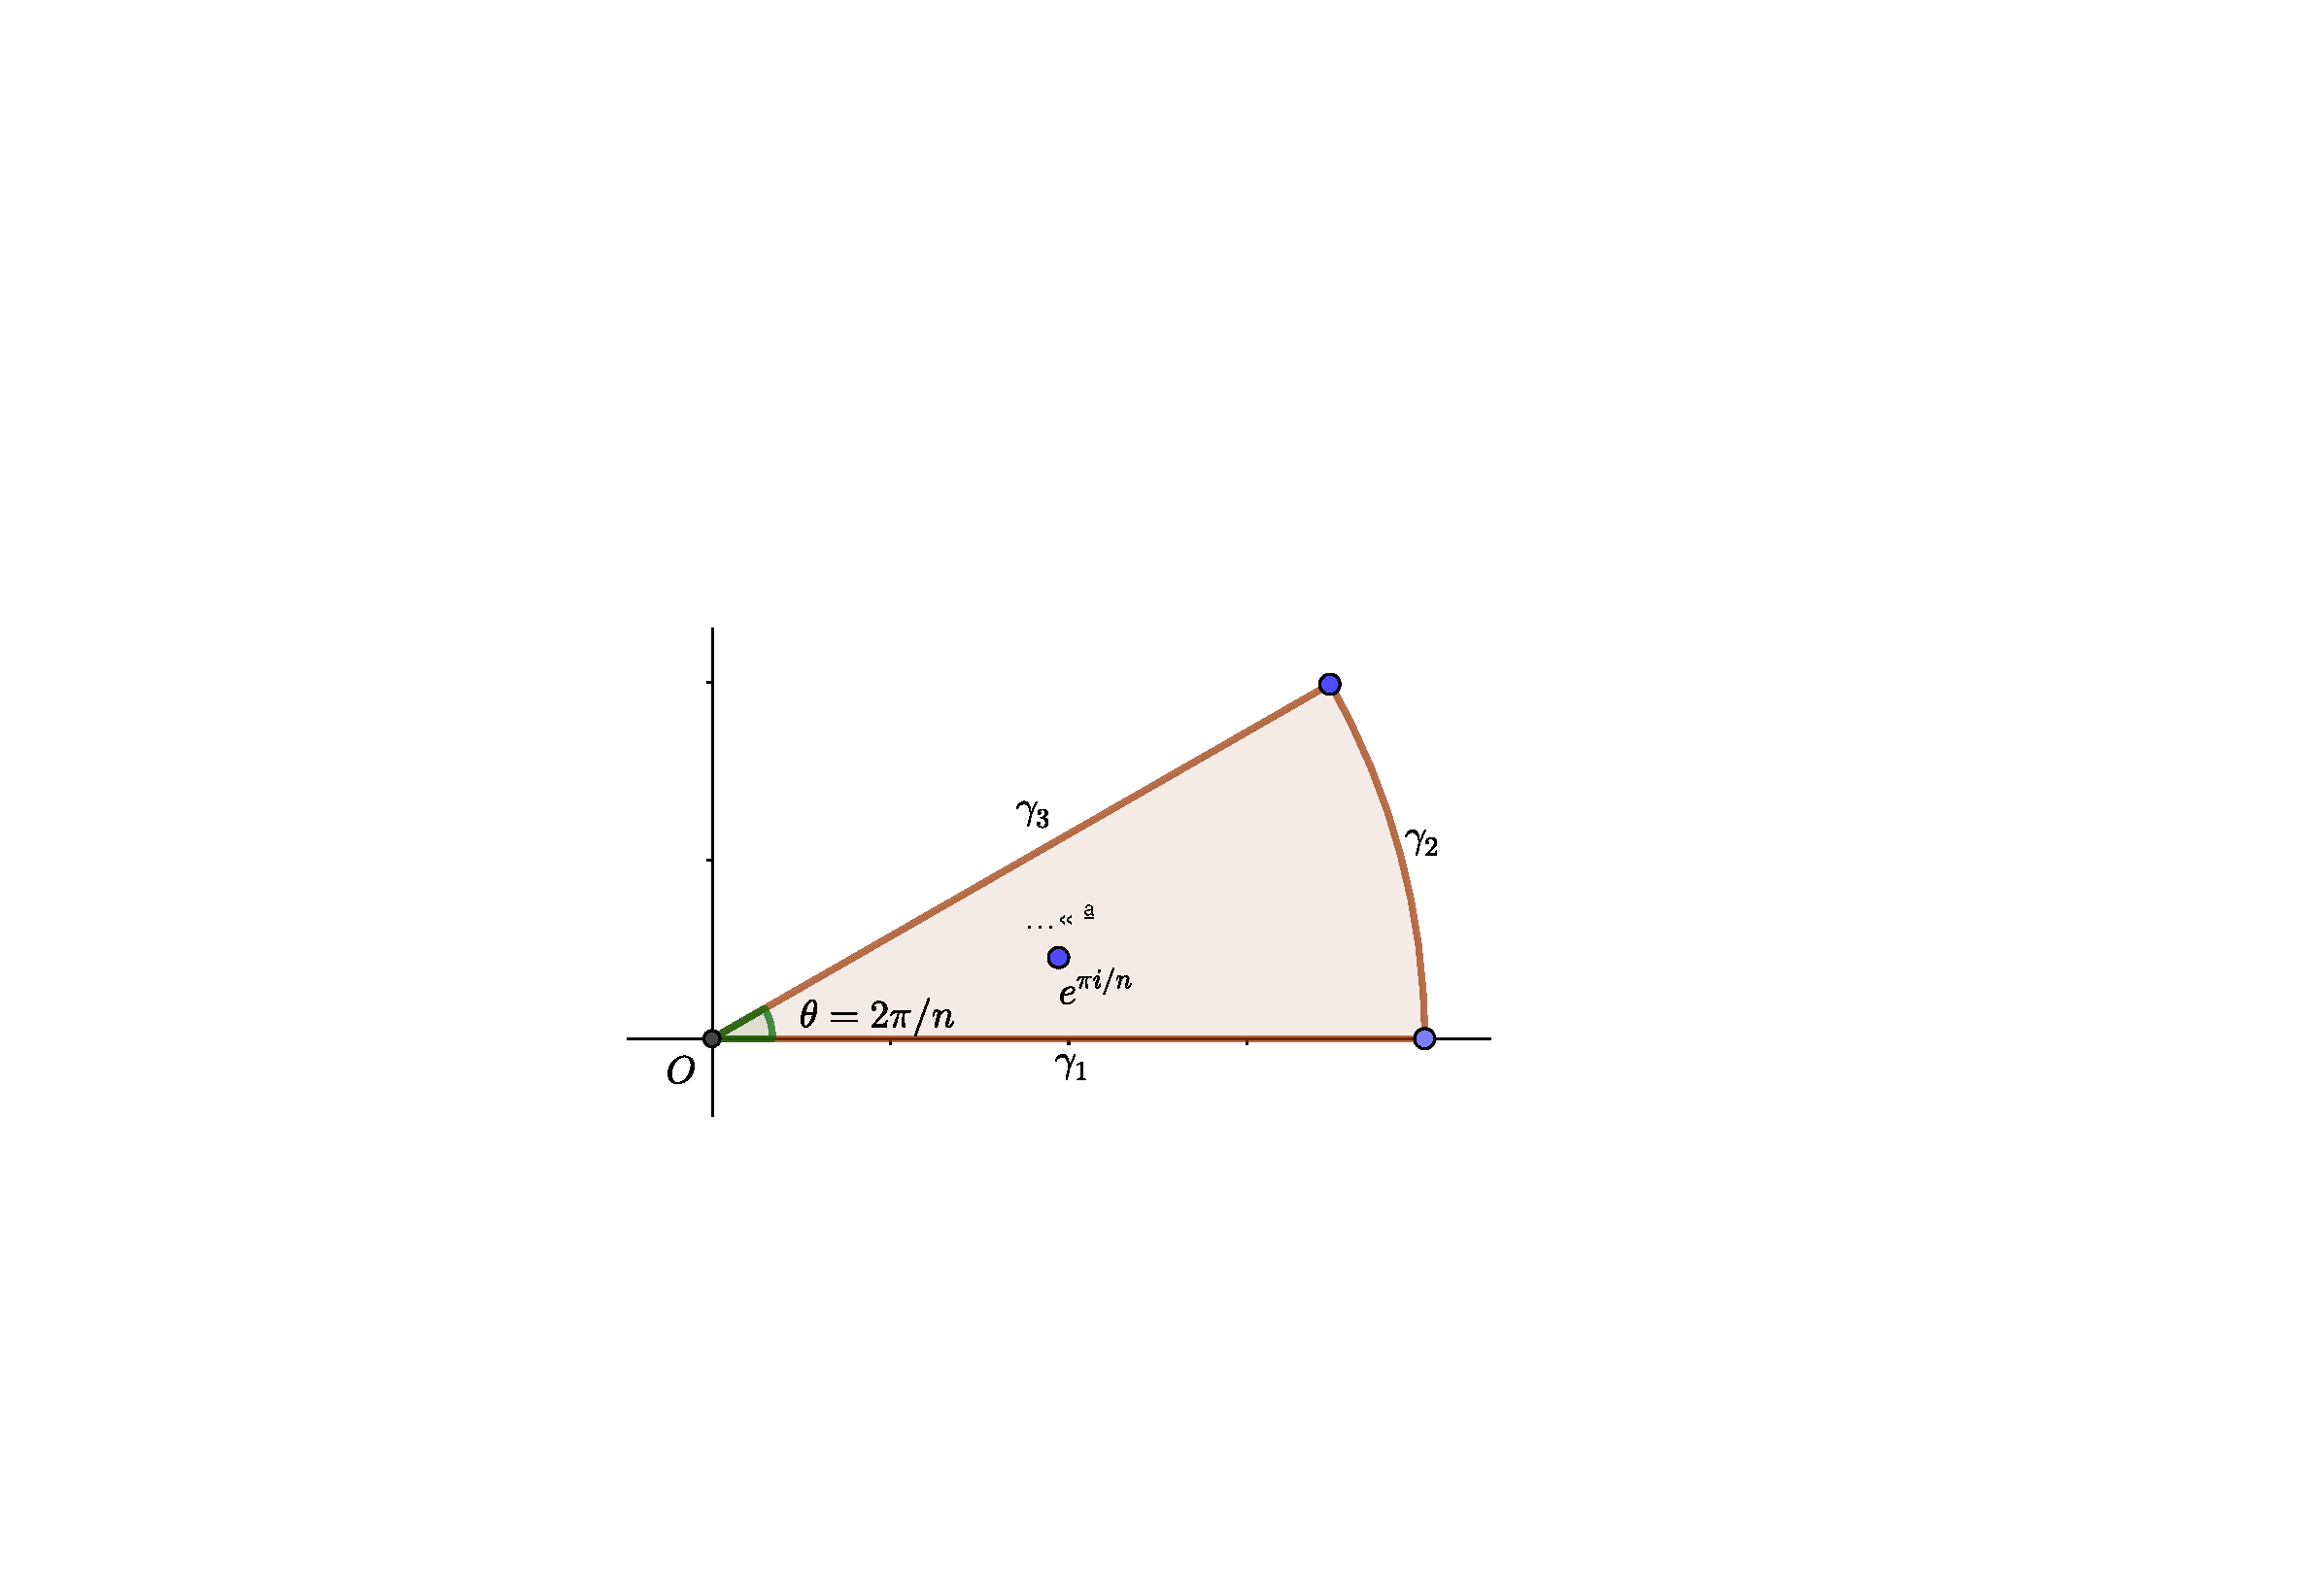
\includegraphics[scale=0.5]{用留数计算1_(1+x^n)在0到正无穷积分.pdf}
    \end{figure}
    
    则$f(z)$在$\gamma$所围成的区域内只有唯一的极点$\e^{\frac{\pi\i}{n}}$, 当$R\to\infty$时

    \begin{align*}
        &\ \int_{\gamma_1} f(z)\,\d z = \int_{0}^\infty \frac{1}{1+x^n}\,\d x,\qquad \int_{\gamma_2}f(z)\,\d z\leq \mathcal{O}\left(\frac{1}{|R|}\right)\to 0,\\
        &\ \int_{\gamma_3} f(z)\,\d z = -e^{\frac{2\pi\i}{n}}\int_0^{\infty}\frac{1}{1+x^n}\,\d x.
    \end{align*}
    则
    \begin{equation*}
        \int_{\gamma}\frac{1}{1+z^n}\,\d z = \left(1-e^{-\frac{2\pi\i}{n}}\right)\int_0^{\infty}\frac{1}{1+x^n}\,\d x,
    \end{equation*}
    由于$\res\left(f;e^{\frac{\pi\i}{n}}\right) = \frac{1}{nz^{n-1}}\biggl|_{z=e^{\frac{\pi\i}{n}}} = \frac{z}{nz^{n}}\biggl|_{z=e^{\frac{\pi\i}{n}}} = -\frac{e^{\frac{\pi\i}{n}}}{n}$ , 所以
    \begin{equation*}
        \int_0^{\infty}\frac{1}{1+x^n}\,\d x = \frac{-\pi\i e^{\frac{\pi\i}{n}}}{n\left(1-e^{\frac{2\pi\i}{n}}\right)} = \frac{-2\pi\i}{n\left(e^{-\frac{\pi\i}{n}}-e^{\frac{\pi\i}{n}}\right)} = \frac{\pi}{n\sin\frac{\pi}{n}}\quad(n\in  \N_{\geq 2}).
    \end{equation*}
\end{proof}
\paragraph{24.}求下列积分:\add

(1) $\int_{0}^{2\pi}\frac{\d\theta}{a-\sin\theta}\ (|a| > 1)$;\qquad(2) $\frac{1}{2\pi}\int_0^{2\pi}\frac{\d \theta}{1-2a\cos\theta+a^2}\ (|a|<1)$.\add

\begin{solution}
    (1) 设$z = \e^{i\theta}$, 则$\sin\theta = \frac{1}{2\i}\left(\e^{\i\theta}-\e^{-\i\theta}\right) = \frac{1}{2\i}\left(z-\frac{1}{z}\right)$, $\d \theta = \frac{\d z}{\i z}$.
    则
    \begin{equation*}
        \int_{0}^{2\pi}\frac{\d\theta}{a-\sin\theta} =\int_{|z|=1}\frac{\d z}{\i z\left(a-\frac{1}{2\i}\left(z-\frac{1}{z}\right)\right)} = 2\int_{|z| = 1}\frac{\d z}{-z^2+2\i az+1},
    \end{equation*}
    方程$-z^2+2\i az+1=0$在$|z|<1$内的根为$\alpha = \i(a-\sqrt{a^2-a})$, 则
    \begin{equation*}
        \int_{0}^{2\pi}\frac{\d\theta}{a-\sin\theta} =2\cdot 2\pi\i\res\left(\frac{1}{-z^2+2\i az+1};\alpha\right) = \frac{2\pi}{\sqrt{a^2-1}}.
    \end{equation*}

    (2) 设$z=\e^{\i \theta}$, 则$\cos \theta = \frac{1}{2}\left(z+\frac{1}{z}\right)$, $\d\theta = \frac{\d z}{\i z}$. 于是
    \begin{equation*}
        \frac{1}{2\pi}\int_{|z| = 1}\frac{\d \theta}{1-2a\cos\theta+a^2} = \frac{1}{2\pi}\int_{|z|=1}\frac{\d z}{\i z\left(1-a\left(z+\frac{1}{z}\right)+a^2\right)} = \frac{1}{2\pi\i}\int_{|z|=1}\frac{\d z}{-az^2+(1+a^2)z-a},
    \end{equation*}
    方程$az^2-(1+a^2)z+a = 0$的根为$\alpha = a, \beta = \frac{1}{a}$, 则$\alpha$在$|z|<1$内, 由留数定理
    \begin{equation*}
        \frac{1}{2\pi}\int_{|z| = 1}\frac{\d \theta}{1-2a\cos\theta+a^2} = \res\left(\frac{1}{-az^2+(1+a^2)z-a};\alpha\right) = \frac{1}{1-a^2}.
    \end{equation*}
\end{solution}
\paragraph{25.}求下列积分:\add

(1) $\int_{0}^\infty\frac{x\sin ax}{x^2+a^2}\,\d x\ (a > 0)$;\qquad (2) $\int_0^{\infty}\frac{\cos x-\e^{-x}}{x}\,\d x$.\add
\begin{solution}
    (1) 构造如图6-10的闭合曲线, 令$f(z) = \frac{z\e^{\i az}}{z^2+a^2}$, 由留数定理
    \begin{equation*}
        \int_{-R}^R\frac{x\e^{\i ax}}{x^2+a^2}\,\d x+\int_{\gamma_R}f(z)\,\d z = 2\pi \i\res\left(f;a\i\right) = \pi\i e^{-a^2},
    \end{equation*}
    由Jordan引理可知, 当$R\to\infty$时, 上式左端第二项为$0$, 所以
    \begin{equation*}
        \int_0^\infty\frac{x\sin ax}{x^2+a^2}\,\d x =\frac{1}{2}\int_{-\infty}^\infty\frac{x\sin ax}{x^2+a^2}\,\d x= \frac{\pi}{2}e^{-a^2}.
    \end{equation*}

    (2) 构造如图6-16的闭合曲线, 虚轴上的积分为
    \begin{equation*}
        \int_{\i R}^{\i r}\frac{\e^{\i z}-\e^{-z}}{z}\,\d z\xlongequal{z\to \i x}-\int_r^R\frac{\e^{-x}-\e^{-\i x}}{x}\,\d x,
    \end{equation*}
    设$f(z) = \frac{\e^{\i z}-\e^{-z}}{z}$, 由Cauchy定理知
    \begin{equation*}
        \int_r^R\frac{\e^{\i x}-\e^{-x}}{x}\,\d x -\int_r^R\frac{\e^{-x}-\e^{-\i x}}{x}\,\d x+\int_{\gamma_r}f(z)\,\d z+\int_{\gamma_R}f(z)\,\d z = 0,
    \end{equation*}
    由于$\lim_{z\to 0}zf(z) = 0$, 由引理1和引理2可知, 当$R\to\infty, r\to0$时, 上式左端第三, 四项为0, 所以
    \begin{equation*}
        \int_0^\infty \frac{\e^{\i x}+\e^{-\i x}-2\e^{-x}}{x}\,\d x = 2\int_0^\infty\frac{\cos x-\e^{-x}}{x}\,\d x =0,
    \end{equation*}
    故$\int_0^\infty\frac{\cos x-\e^{-x}}{x}\,\d x =0$.
\end{solution}
\paragraph{26.}求下列积分:
(1) $\int_0^{\infty}\frac{\log x}{x^2-1}\,\d x$;\qquad (2) $\int_0^{\infty}x^{p-1}\cos x\,\d x\ (0 < p < 1)$.\add
\begin{solution}
    (1) 构造如下图所示的闭合曲线$\gamma = \mathrm{I}+\mathrm{II}+\mathrm{III}+\gamma_r+\gamma_R$.
    \begin{figure}[htbp]
        \centering
        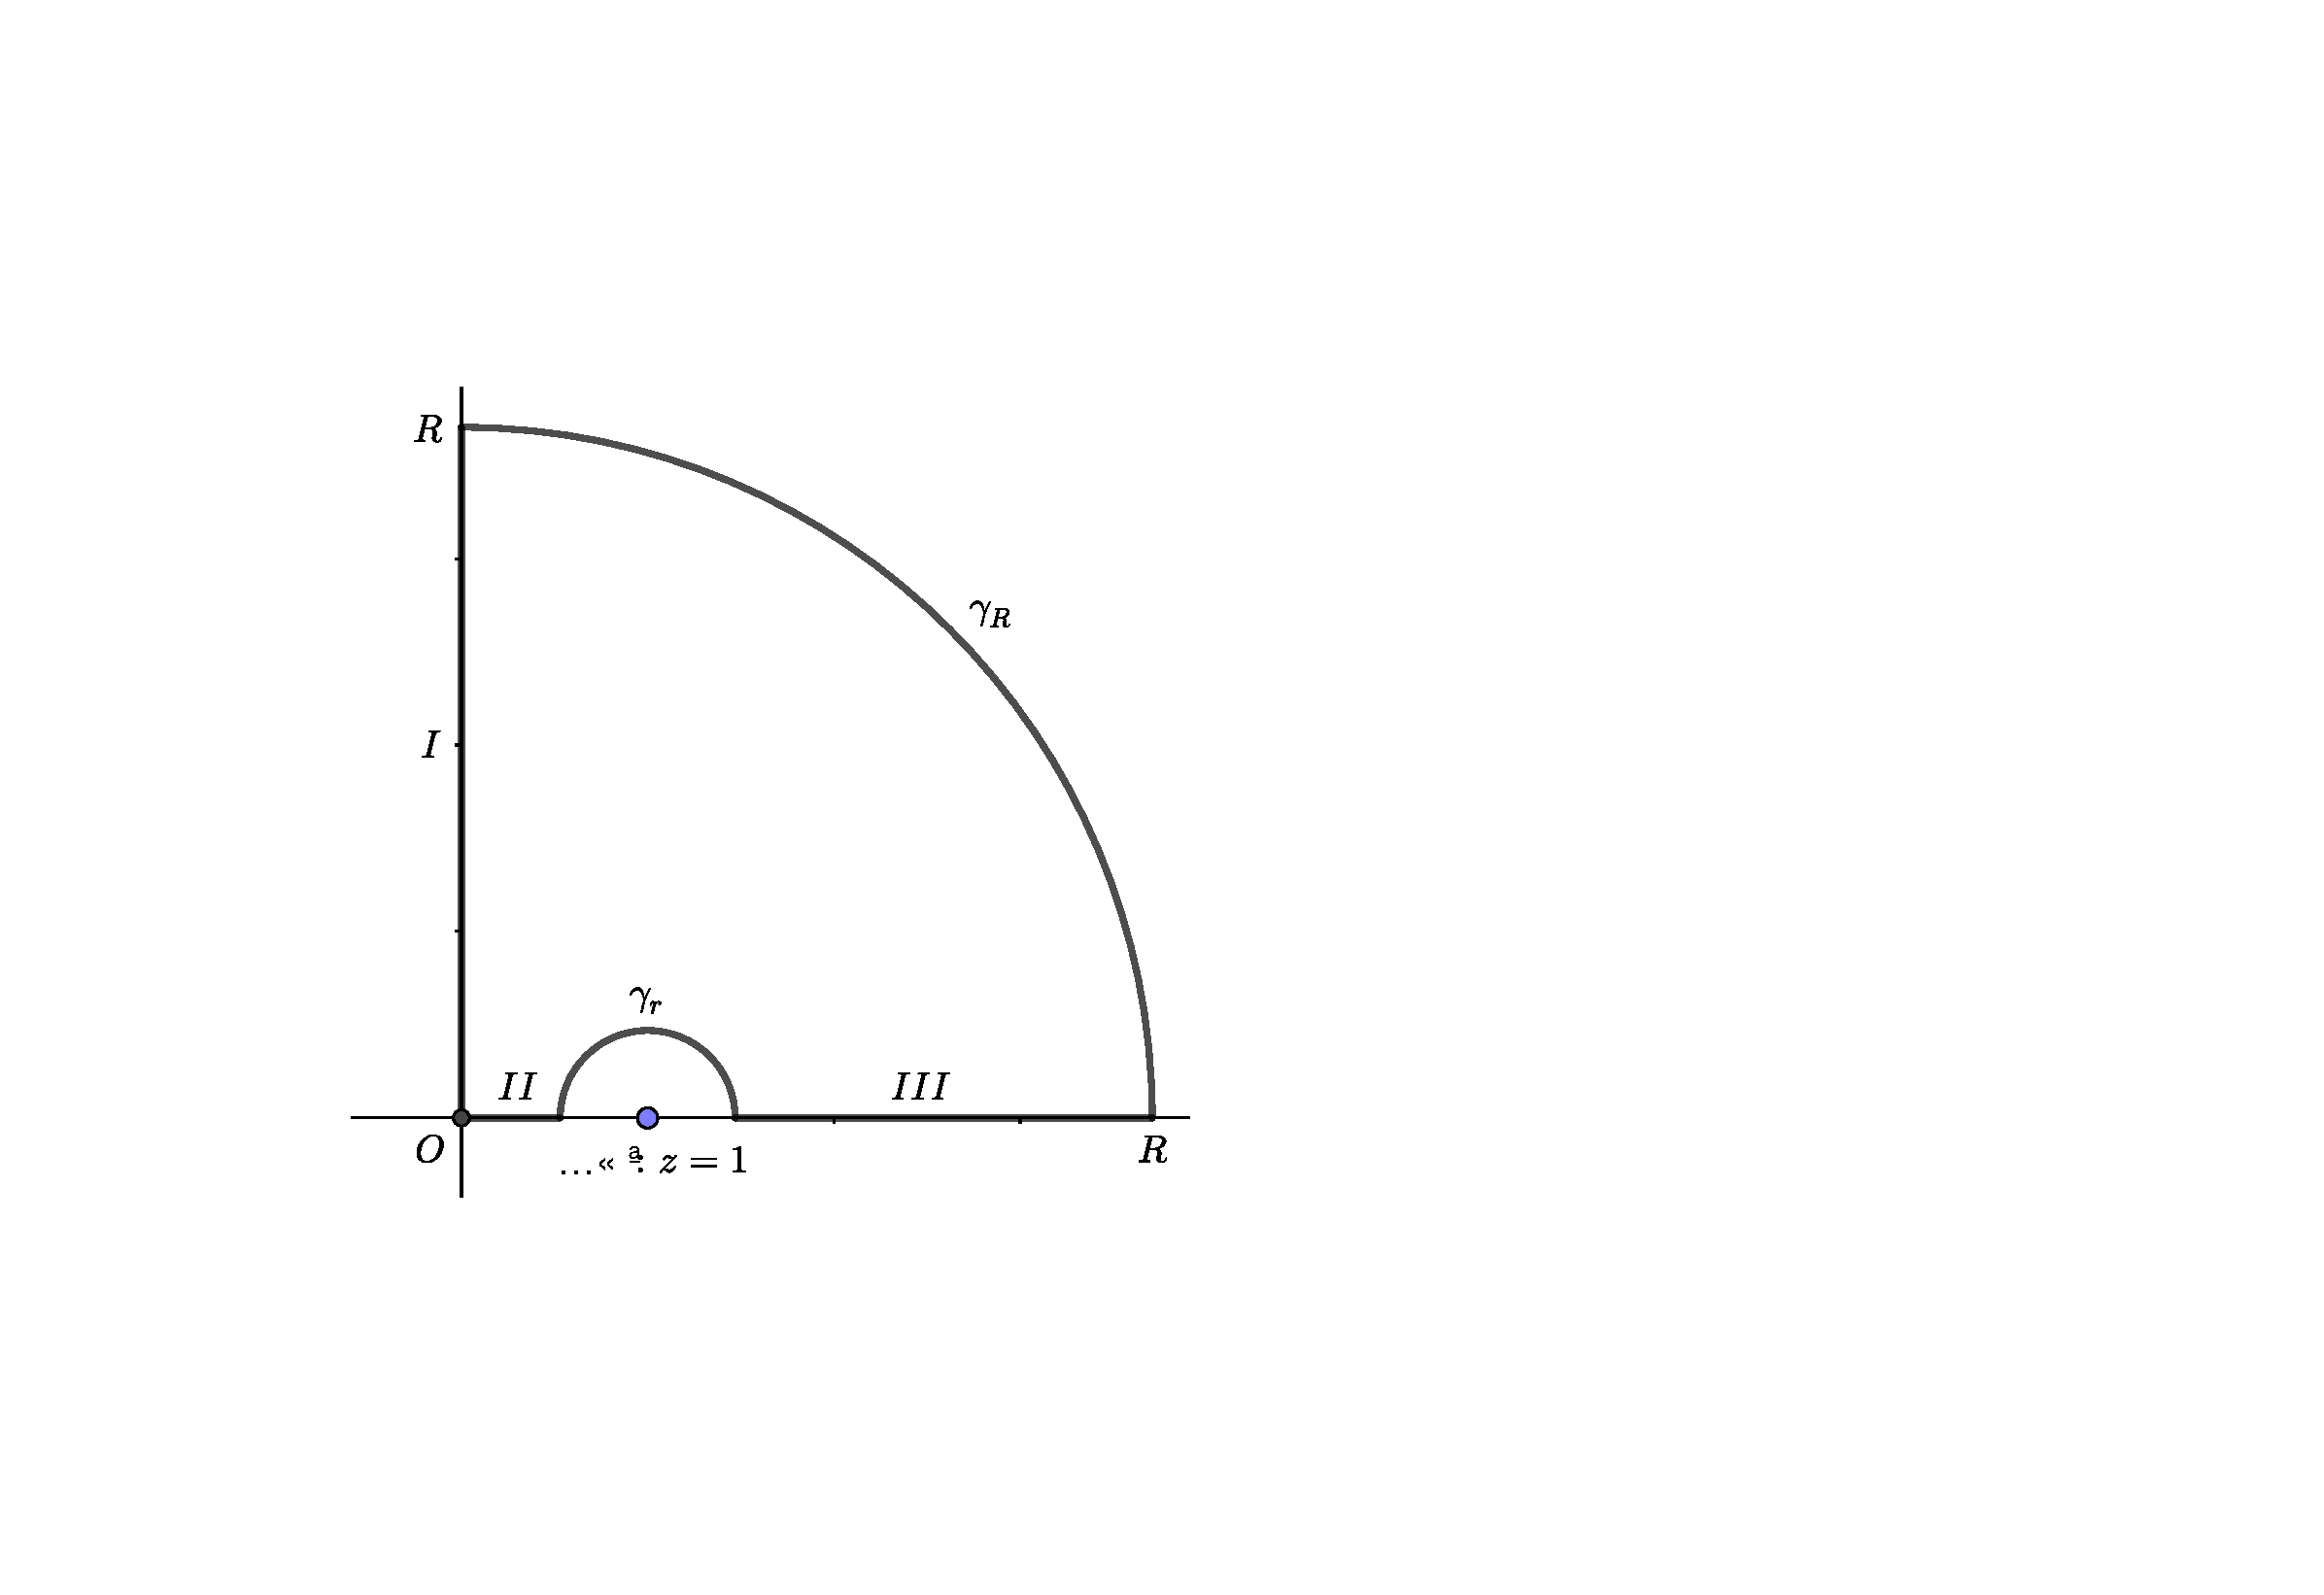
\includegraphics[scale=0.5]{留数计算logx_(x^2-1) 0到inf上的积分.pdf}
    \end{figure}
    设$f(z) = \frac{\log z}{z^2-1}$, 由于$z=1$为$f(z)$的一级极点, 且$\lim_{z\to 1}(z-1)f(z) = 0$, 由引理1可知$\int_{\gamma_r}f(z)\,\d z = 0$; 又由于
    \begin{equation*}
        \left|\int_{\gamma_R}\frac{\log z}{z^2-1}\,\d z\right|\leq \int_0^{\frac{\pi}{2}}\frac{R\log R}{R^2\e^{2\i\theta}-1}\,\d \theta\to 0\quad(R\to\infty).
    \end{equation*}

    在路径$I$上, $z=\i y\ (0\leq y\leq R)$, 则
    \begin{equation*}
        \int_I\frac{\log z}{z^2-1}\,\d z = - \frac{\pi}{2}\int_0^R\frac{\d y}{y^2+1} = -\frac{\pi}{2}\arctan R.
    \end{equation*}

    于是当$R\to\infty,\ r\to 0$时, 由Cauchy定理知
    \begin{align*}
        &\ \int_{\mathrm{I}}f(z)\,\d z+\int_{\mathrm{II}}f(z)\,\d z+\int_{\mathrm{III}}f(z)\,\d z+\int_{\mathrm{\gamma_r}}f(z)\,\d z+\int_{\mathrm{\gamma_R}}f(z)\,\d z = 0\\
        \Rightarrow&\ \int_{0}^\infty\frac{\log x}{x^2-1}\,\d x = -\int_{I}f(z)\,\d z = \left(\frac{\pi}{2}\right)^2.
    \end{align*}

    (2) 构造如图6-16的闭合曲线, 设$f(z) = z^{p-1}\e^{\i z}$, 则在$\gamma_R$上
    \begin{equation*}
        \int_{\gamma_{R}}f(z)\,\d z \xlongequal{z = R\e^{\i \theta}} \i R^{p}\int_{0}^{\frac{\pi}{2}}\e^{\i p\theta}\e^{\i R\cos\theta}\e^{-R\sin\theta}\,\d \theta,
    \end{equation*}
    于是
    \begin{equation*}
        \left|\int_{\gamma_R}f(z)\,\d z\right| \leq R^p\int_0^{\frac{\pi}{2}}\e^{-R\sin\theta}\,\d \theta\leq  R^{p}\int_0^{\frac{\pi}{2}}\e^{-\frac{2R}{\pi}\theta}\,\d\theta = \frac{\pi}{2R^{1-p}}\left(1-\e^{-R}\right)\to 0\quad(R\to\infty).
    \end{equation*}
    类似地, 在$\gamma_r$上
    \begin{equation*}
        \left|\int_{\gamma_r}f(z)\,\d z\right| \leq \frac{\pi}{2r^{1-p}}\left(\e^{-r}-1\right)\to 0\quad(r\to 0).
    \end{equation*}
    在虚轴部分上, $z = \i y\ (r\leq y\leq R)$, 于是
    \begin{equation*}
        \int_R^r(\i y)^{p-1}\e^{-y}\i\,\d y =-\i^p\int_r^Ry^{p-1}\e^{-y}\,\d y\xlongequal{\i = \e^{\frac{\pi}{2}\i}} -\e^{\frac{\i \pi p}{2}}\int_r^Ry^{p-1}\e^{-y}\,\d y,
    \end{equation*}
    令$R\to\infty,\ r\to 0$, 由Cauchy定理知
    \begin{equation*}
        \int_0^{\infty}x^{p-1}\e^{\i x}\,\d x = \e^{\frac{\i\pi p}{2}}\int_0^{\infty}y^{p-1}\e^{-y}\,\d y = \Gamma(p)\cos \frac{\pi p}{2}+\i\Gamma(p)\sin \frac{\pi p}{2},
    \end{equation*}
    取实部可得
    \begin{equation*}
        \int_0^{\infty}x^{p-1}\cos x\,\d x = \Gamma(p)\cos\frac{\pi p}{2}.
    \end{equation*}
\end{solution}\del
\paragraph{27.}计算积分$\int_0^\infty\e^{-x^2}\cos x^2\,\d x$.
\begin{solution}
    构造如图6-12的曲线, 其中$\mathrm{II} = x\e^{\frac{\pi}{8}\i}$, 设$f(z) = \e^{-(1-\i)z^2}$, 则在$\gamma_R$上
    \begin{align*}
        \left|\int_{\gamma_R}\e^{-(1-\i)z^2}\,\d z\right|\leq&\ R\int_0^{\frac{\pi}{8}}\e^{-R^2(\cos2\theta+\sin2\theta)} =R\int_0^{\frac{\pi}{8}}\e^{-\sqrt{2}R^2\sin(\frac{\pi}{4}+2\theta)}\,\d \theta\\
        \leq&\ R\int_0^{\frac{\pi}{8}}\e^{-\frac{\pi}{2}R^2}\e^{-\frac{4\sqrt{2}R^2}{\pi}\theta}\,\d \theta\leq \frac{\pi}{4\sqrt{2}R}\e^{-\frac{\sqrt{2}}{2}R^2} \to 0\quad(R\to\infty).
    \end{align*}
    在$\mathrm{II}$上, $z = x\e^{\frac{\pi}{8}\i}$, 于是
    \begin{equation*}
        \int_{\mathrm{II}}f(z)\,\d z = \frac{-1}{\sqrt{1-\i}}\int_0^R\e^{-x^2}\,\d x,
    \end{equation*}
    当$\R\to\infty$时, 由Cauchy定理知
    \begin{equation*}
        \int_0^{\infty}\e^{-x^2}\e^{\i x^2}\,\d x = \frac{1}{2}\sqrt{\frac{\pi}{1-\i}} = \frac{1}{2}\sqrt{\frac{\pi}{\sqrt{2}}}\e^{\frac{\pi}{8}\i},
    \end{equation*}
    取实部可得
    \begin{equation*}
        \int_0^\infty\e^{-x}\cos x\,\d x = \frac{\sqrt{\pi(1+\sqrt{2})}}{4}.
    \end{equation*}
\end{solution}

% 下面给一些功能的写法
\iffalse
% 图片模板
\centerline{
    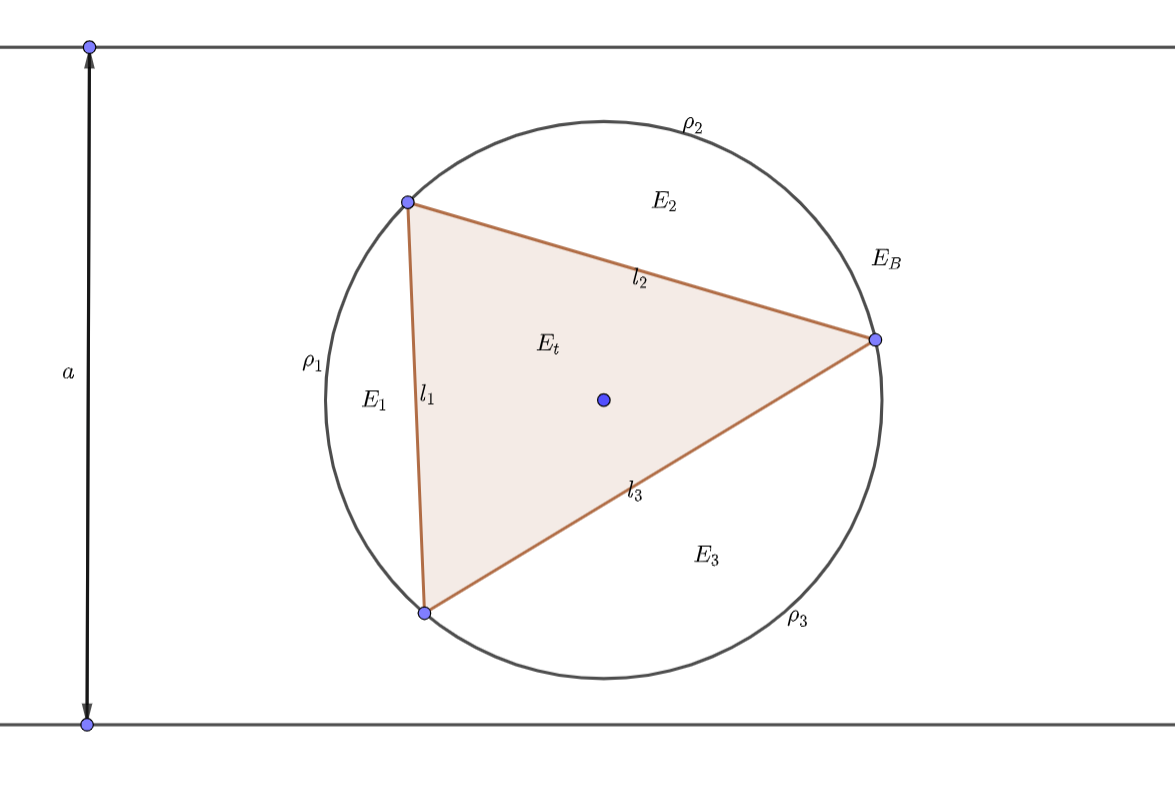
\includegraphics[width=0.8\textwidth]{figure.png}
}
% 表格模板
\renewcommand\arraystretch{0.8} % 设置表格高度为原来的0.8倍
\begin{table}[!htbp] % table标准
    \centering % 表格居中
    \begin{tabular}{p{1cm}<{\centering}p{1cm}<{\centering}p{3cm}<{\centering}p{5cm}<{\centering}} % 设置表格宽度
    %\begin{tabular}{cccc}
        \toprule
        $x_i$ & $f[x_1]$ & $f[x_i,x_{i+1}]$ & $f[x_i,x_{i+1},x_{i+2}]$ \\
        \midrule
        $x_0$ & $f(x_0)$ &                  &                          \\
        $x_0$ & $f(x_0)$ & $f'(x_0)$        &                          \\
        $x_0$ & $f(x_1)$ & $\frac{f(x_1)-f(x_0)}{x_1-x_0}$ & $\frac{f(x_1)-f(x_0)}{(x_1-x_0)^2}-\frac{f'(x_0)}{x_1-x_0}$\\
        \bottomrule
    \end{tabular}
\end{table}

\def\Log{\text{Log}} % 一个简单的宏定义
$\Log$ % 调用方法
\fi

\end{document}